\documentclass[twocolumn,10pt]{asme2e}
\special{papersize=8.5in,11in}

\usepackage{graphicx}
\usepackage{amsmath,amssymb}
\usepackage{amsfonts}
\usepackage{url}
\usepackage{nth}
\usepackage[hidelinks]{hyperref}
\usepackage{flushend}
%\confshortname{IDETC/CIE 2009}
%\conffullname{the ASME 2009 International Design Engineering Technical Conferences \&\\
%	Computers and Information in Engineering Conference}

%%%%% for date in a single month, use
%\confdate{24-28}
%\confmonth{September}
%%%%% for date across two months, use
%\confdate{August 30-September 2}
%\confyear{2009}
%\confcity{San Diego}
%\confcountry{USA}

%%% Replace DETC2009/MESA-12345 with the number supplied to you 
%%% by ASME for your paper.
\papernum{CS289A Course Project}

%%% You need to remove 'DRAFT: ' in the title for the final submitted version.
\title{Short-term freeway traffic prediction using neural networks}

%%% first author
\author{Negar Zahedimehr\thanks{SID: 24984323}
	\affiliation{
		Department of Mechanical Engineering\\
		University of California\\
		Berkeley, California 94720\\
		Email: negar.mehr@berkeley.edu
	}	
}

%%% second author
%%% remove the following entry for single author papers
%%% add more entries for additional authors
\author{Behrooz Shahsavari \thanks{SID: 23260557}
	\affiliation{Department of Mechanical Engineering\\
		University of California\\
		Berkeley, California 94720\\
		Email: behrooz@berkeley.edu
	}
}

\begin{document}
	
	\maketitle

\maketitle    

%%%%%%%%%%%%%%%%%%%%%%%%%%%%%%%%%%%%%%%%%%%%%%%%%%%%%%%%%%%%%%%%%%%%%%
\begin{abstract}
{\it 
	This paper proposes a fully automated method for simulating/predicting freeway traffic data by deploying neural networks. Our emphasis is on predicting ``{speed}", ``{occupancy}" and ``{flow}" of freeway segments by training neural networks using data provided by a set of sensors called ``{loop detectors}" that are being implemented in the freeway system of the state of California. This data is obtained from Caltrans Performance Measurement System  that collects real-time data from over 39,000 individual detectors.
	The main advantage of attaining a neural network representing freeway traffic behavior is that it eliminates the need to assume a rule governing dynamics of traffic; thus, eradicates the process of parameter estimation. Besides, we have shown that very complicated traffic behavior, such as time-dependent nature of it can be captured by a neural network, e.g. by considering time as one of the inputs to the model. 
	We also discuss deploying unsupervised learning classification algorithms for removing ``false" data in the preprocessing stage to avoid this type of data in our neural network training.
}
\end{abstract}

\section{Introduction}

\par Macroscopic traffic models are widely used by transportation engineers in order to design controllers and perform re-routing or road management to improve performance of the system such as increasing total traveled distance and decreasing total travel time of vehicles in the network. Macroscopic models deal with large-scale properties of vehicular networks rather than intricacies of lower impact on the wide-ranging performance of a network such as modeling drivers' behavior. As a matter of fact, these models are complex enough to capture network-wide properties of the system and simple enough to be capable of performing real-time operations \cite{MacroModels}.

When it comes to planning and management of intelligent transportation systems (ITS), short-term and long-term predictions of traffic behavior and pattern, play a key role \cite{TrafficPrediction}. An immense amount of research has been conducted on how to come up with accurate short-term predictions of traffic. Nearest neighbor techniques \cite{nearestNeighbor}, Kalman filtering \cite{Kalman} and spectral and cross-spectral analyses \cite{spectral} are some instances of traffic flow prediction approaches taken by researchers. Generally, the traditional procedure of traffic prediction consists of discovering the rules that presumably govern and model dynamics and evolution of traffic, estimation of required parameters of the acquired dynamics and then letting the traffic model evolve by obtained model of estimated parameters to make a prediction.   

A burdensome aspect of traffic prediction is that traffic pattern and behavior is contingent on too many different variables and conditions. As an illustration, for a given network, the day for which prediction is required, plays a significant role as traffic regime on weekends may vary from the one on workdays. Furthermore, even for a particular day, clearly, vehicular traffic in evenings differs from the one at midnight since there may be a huge number of commuters at particular hours of a day. Thus, a decent traffic prediction must incorporate distinct parameters influencing traffic conditions. In order for a model-based prediction to have acceptable performance under various conditions, the task of estimation of model's parameters should be repeated once traffic regime is altering. It may even be more exhausting to perceive the situations when re-estimation of parameters is needed. 
%\section{Motivation}

Transportation engineers normally divide study of vehicular networks into two pieces, urban arterial networks and freeways as traffic behaves distinctly in these networks. The latter is the focus of this study. 
As every watchful motorist driving in California freeways can recognize, there are numerous implemented loop detectors in freeway stretches of California that measure and record traffic metrics. These sensors provide traffic data-centers with huge amount of information that must be taken into account while making predictions. The immense existing data and complexity of traffic behavior as a result of being affected by different continuous and discrete variables, motivated the authors to perform traffic prediction deploying neural network and deep learning methods to come up with a traffic prediction which can possibly perform better than the existing traffic predictors\cite{NNreview}. The main advantage of attaining a neural network representing freeway traffic behavior is that it eliminates the need to assume a rule governing dynamics of traffic; thus, eradicates the process of parameter estimation. Besides, complexities of the model such as time-dependent nature of traffic is captured by the neural network internally as time is considered as one of the inputs of the system. 
\section{Macroscopic Freeway Models}
In macroscopic freeway traffic models, large-scale properties of the network influential in planning are considered. Commonly, these models step on two components: \emph{vehicular densities} and \emph{vehicular flow} where the first term refers to number of vehicles in a partition of space and the latter is interpreted as the number of vehicles leaving a particular segment of freeway. 
The most prevalent first-order freeway model presumed to determine dynamics of freeway and extensively in use is Cell Transmission Model \cite{CTM} in which freeway is divided into $N$ segments called \emph{links}  such that each link has at most one on-ramp and one off-ramp. For a given link $i$ at time $k$, state (vehicular density) of the link $i$ is updated by equation \ref{CTM_update} where $n_i(k)$ is the density of vehicles in section $i$ at time $k$, $f_i(k)$ is the flow leaving section $i$ at time $k$ and  $f_{i-1}(k)$ is the flow entering section $i$ from section $i-1$. Equation \ref{CTM_update} indicates that each link is coupled to the adjacent links through the flows entering and exiting links. 
In order to let equation \ref{CTM_update} represent the observed behavior of a given freeway, there must be a function mapping flow at each section to its density. This mapping function is called a \textit{fundamental diagram}.
\begin{equation} \label{CTM_update}
n_i(k+1) = n_i(k) - f_i(k) + f_{i-1}(k)
\end{equation}

\subsection{Fundamental Diagrams}
Macroscopic models take advantage of the assumption of existence of a fundamental diagram for each link in the freeway depicting the relationship between observed vehicular flow in the link and its vehicular density \cite{Calibration}. Generally, in order to obtain the fundamental diagram for a given link, vehicular density and flow of that link are recorded for various traffic conditions and the best possible curve is fitted to the observed data \cite{cassidy}. In first order freeway traffic models, a piece-wise linear function is fitted to the data as shown in figure \ref{fig:fd}. Consideration of a piece-wise linear function implies that flow in a link is restricted to be in three different regimes: \textit{free-flow} region which is the left side of the triangular shape with a positive slope ($v_i$), flow being equal to \textit{capacity} ($F_i$) which is the maximum flow that can leave a section (peak point in piece-wise linear function) and \textit{congested} region corresponding to the right side of the triangular shape with negative slope ($w_i$). Equivalently, flow is calculated according to equation \ref{flow_equation} where $\bar{n}$ is the jam density or maximum number of vehicles a link can accommodate. The \textit{min} term in equation \ref{flow_equation} suggests that freeway dynamics is dictated by a non-linear law.
\begin{equation} \label{flow_equation}
f_i(k) = \min \big( v_in_i(k), F_i(k), w_{i+1}(\bar{n}_{i+1} - n_{i+1}(k))\big)
\end{equation}

\subsection{Calibration}
The aforementioned coupling and non-linearity of freeway models insinuate that calibration of fundamental diagram for each link must be performed such that traffic behavior is consistent all over the network; in other words, calibrated fundamental diagram of a link may not be accurate enough by considering isolated flow-density relation of the corresponding link. On the other hand, parameters of a fundamental diagram vary over time since traffic regime alters during the day. In order for a simulation by a macroscopic model to represent traffic behavior, the assigned fundamental diagrams are tuned so as to find the set of fundamental diagrams yielding to trajectories close to the observed traffic trajectories which is of course a cumbersome process. Furthermore, due to the time-varying nature of traffic, the whole process should be repeated for different time intervals during which traffic parameters are supposed to be constant \cite{Calibration}. 

\begin{figure}[h]
    \centering
    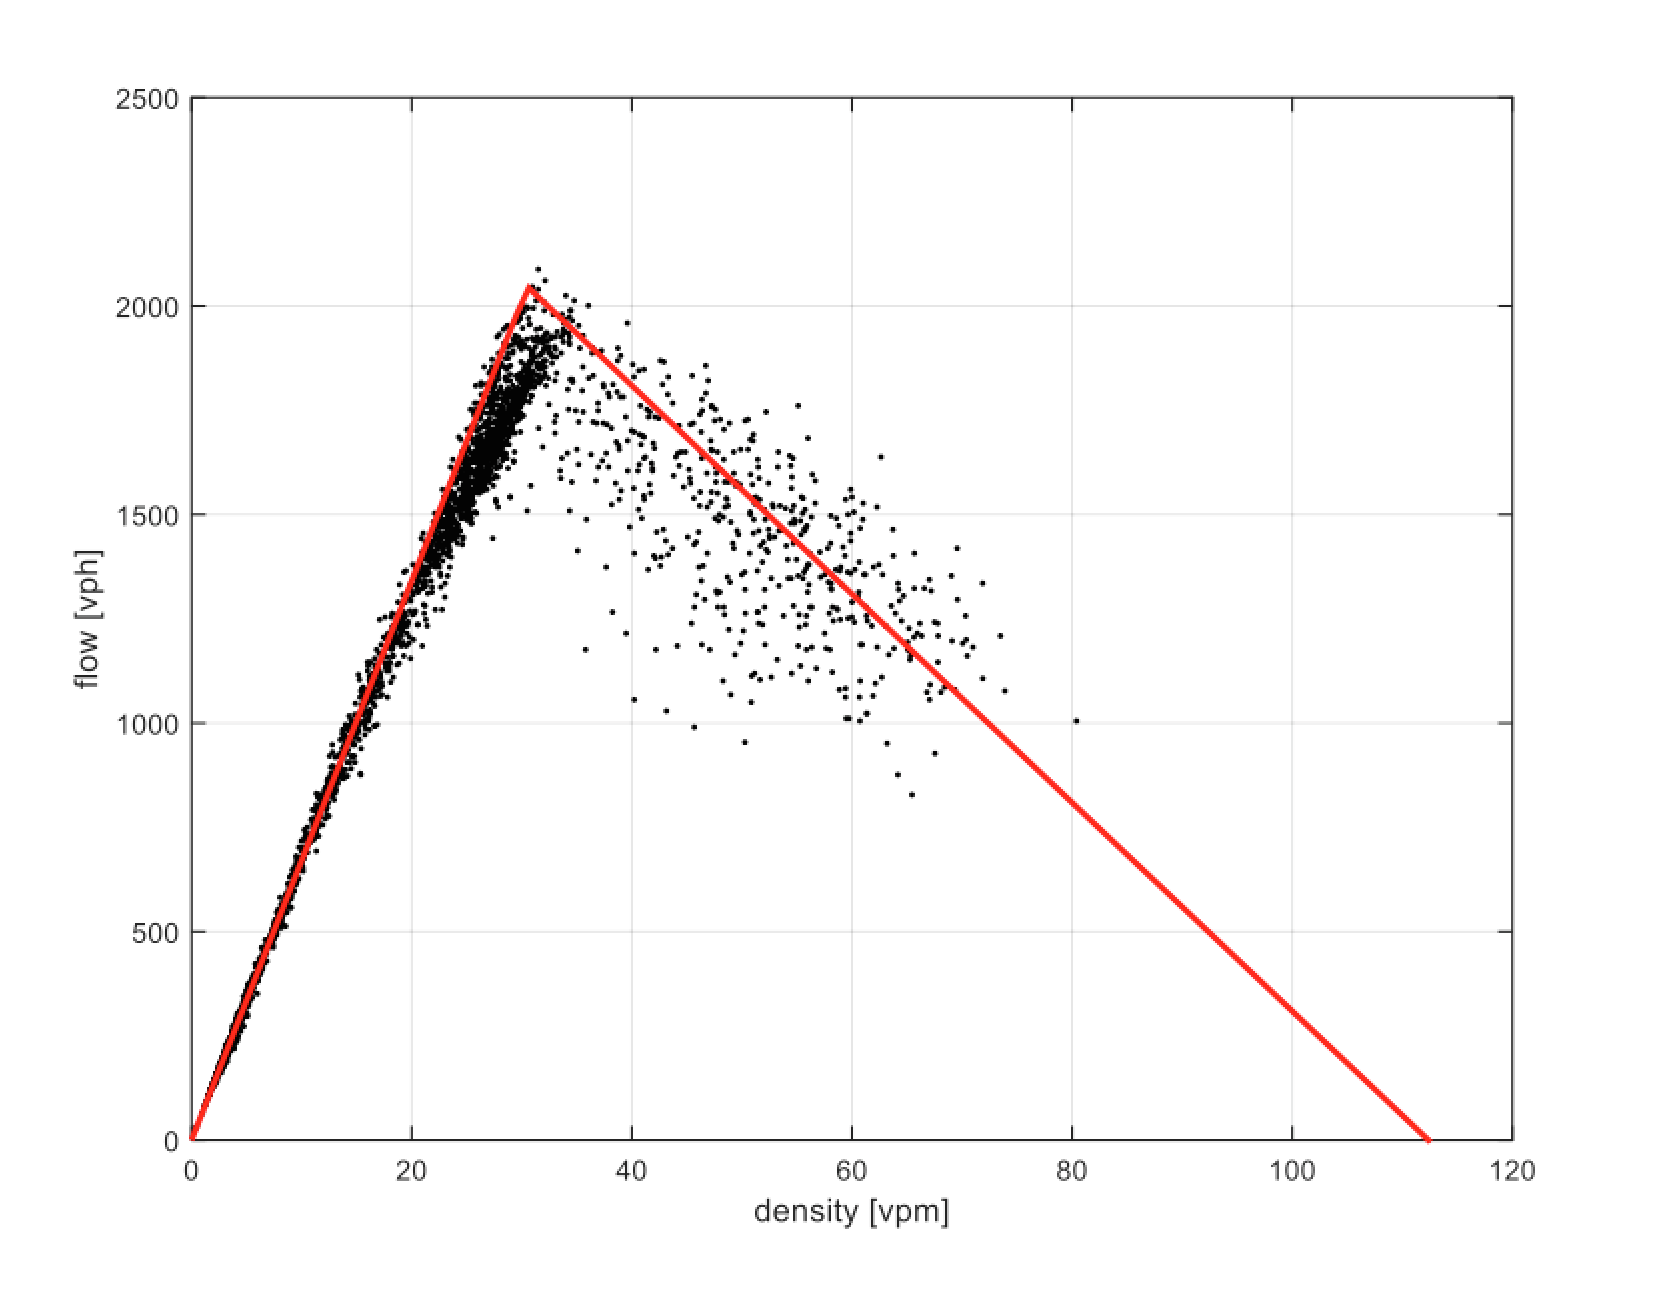
\includegraphics[width=0.8\linewidth]{fd.png}
    \caption{Fundamental Diagram of a Link in I-210 east}
    \label{fig:fd}
\end{figure} 
\subsection{Inspiration}
The aforestated complexities of conventional macroscopic simulators led the authors to exploit the massive amount of traffic data to go beyond fundamental diagrams and piece-wise affine dynamics of CTM and perceive a multi-input multi-output function for short-term traffic prediction in which time of the day and day of week are taken into account as inputs as well. Clearly, the dynamics and evolution of traffic variables is captured by the recorded data regardless of whether there exists a triangular fundamental diagram dictating flow-density relations for a given link or not, revealing the fact that there is no need for burdensome process of calibration or estimation of model parameters. Moreover, prediction performance and accuracy can perhaps improve; for, extra information such as date and time are provided to the trained multi-layer neural network model \cite{neuralForcast}.  


\section{Data Analysis}
\subsection{Training Data} 
PeMS (Performance Measurement System) is a traffic metrics measurement system spanning freeway system across state of California deployed to obtain loop detector data in real time \cite{PemsPravin}. Freeway PeMS data consists of the following measurements on time intervals of $5$ minutes:
\begin{itemize}
\item[1]\textbf{Vehicular Flow}: Number of vehicles crossing a sensor 
\item[2]\textbf{Occupancy}: Fraction of time a vehicle is present on the loop detector\cite{occupancy}.
\item[3]\textbf{Speed}: The rate with which vehicles cross a loop detector.

\end{itemize}

PeMS data is available to users at \url{http://pems.dot.ca.gov/}. In this project, Freeway I-210 East (Figure \ref{fig:210}) PeMS data was used as the training and validation data set. Each day is divided into 288 intervals where each time interval lasts $5$ minutes. The data used in this project was collected for the last three months of 2014 (October 1\textsuperscript{st} to December 31\textsuperscript{st}).
\begin{figure}[h]
    \centering
    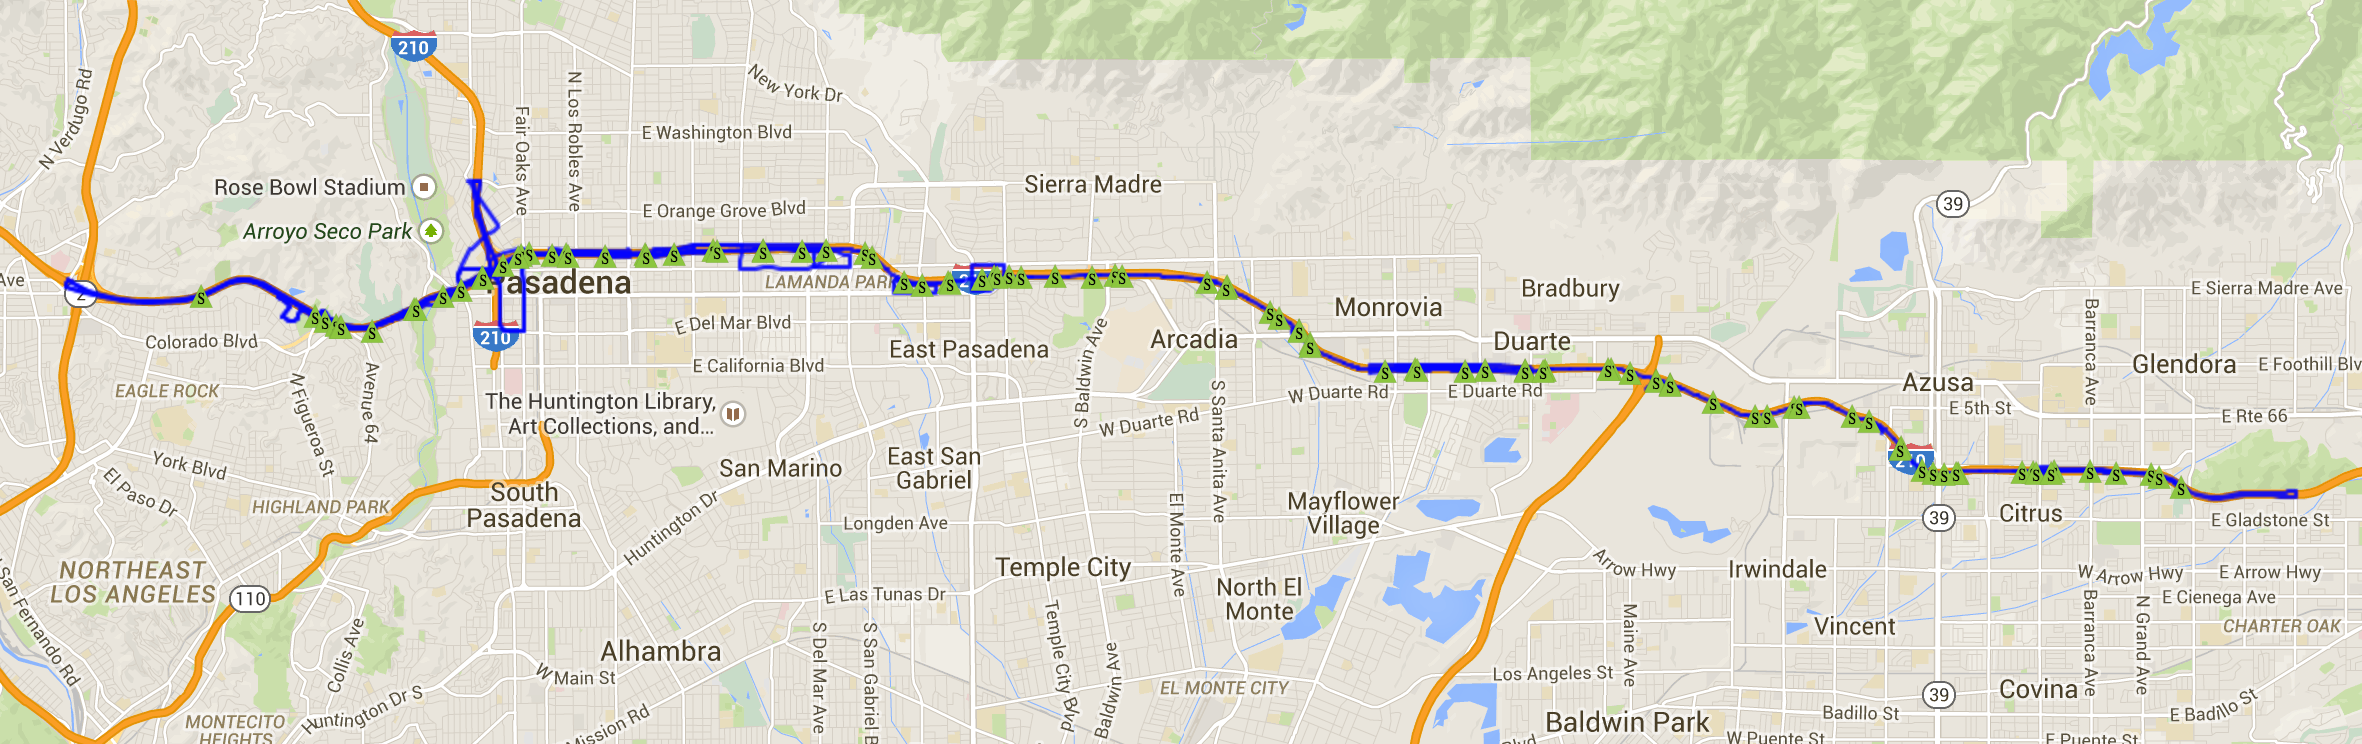
\includegraphics[width=1\linewidth]{210.png}
    \caption{I-210 East Topology}
    \label{fig:210}
\end{figure} 

\begin{figure}[h]
	\centering
	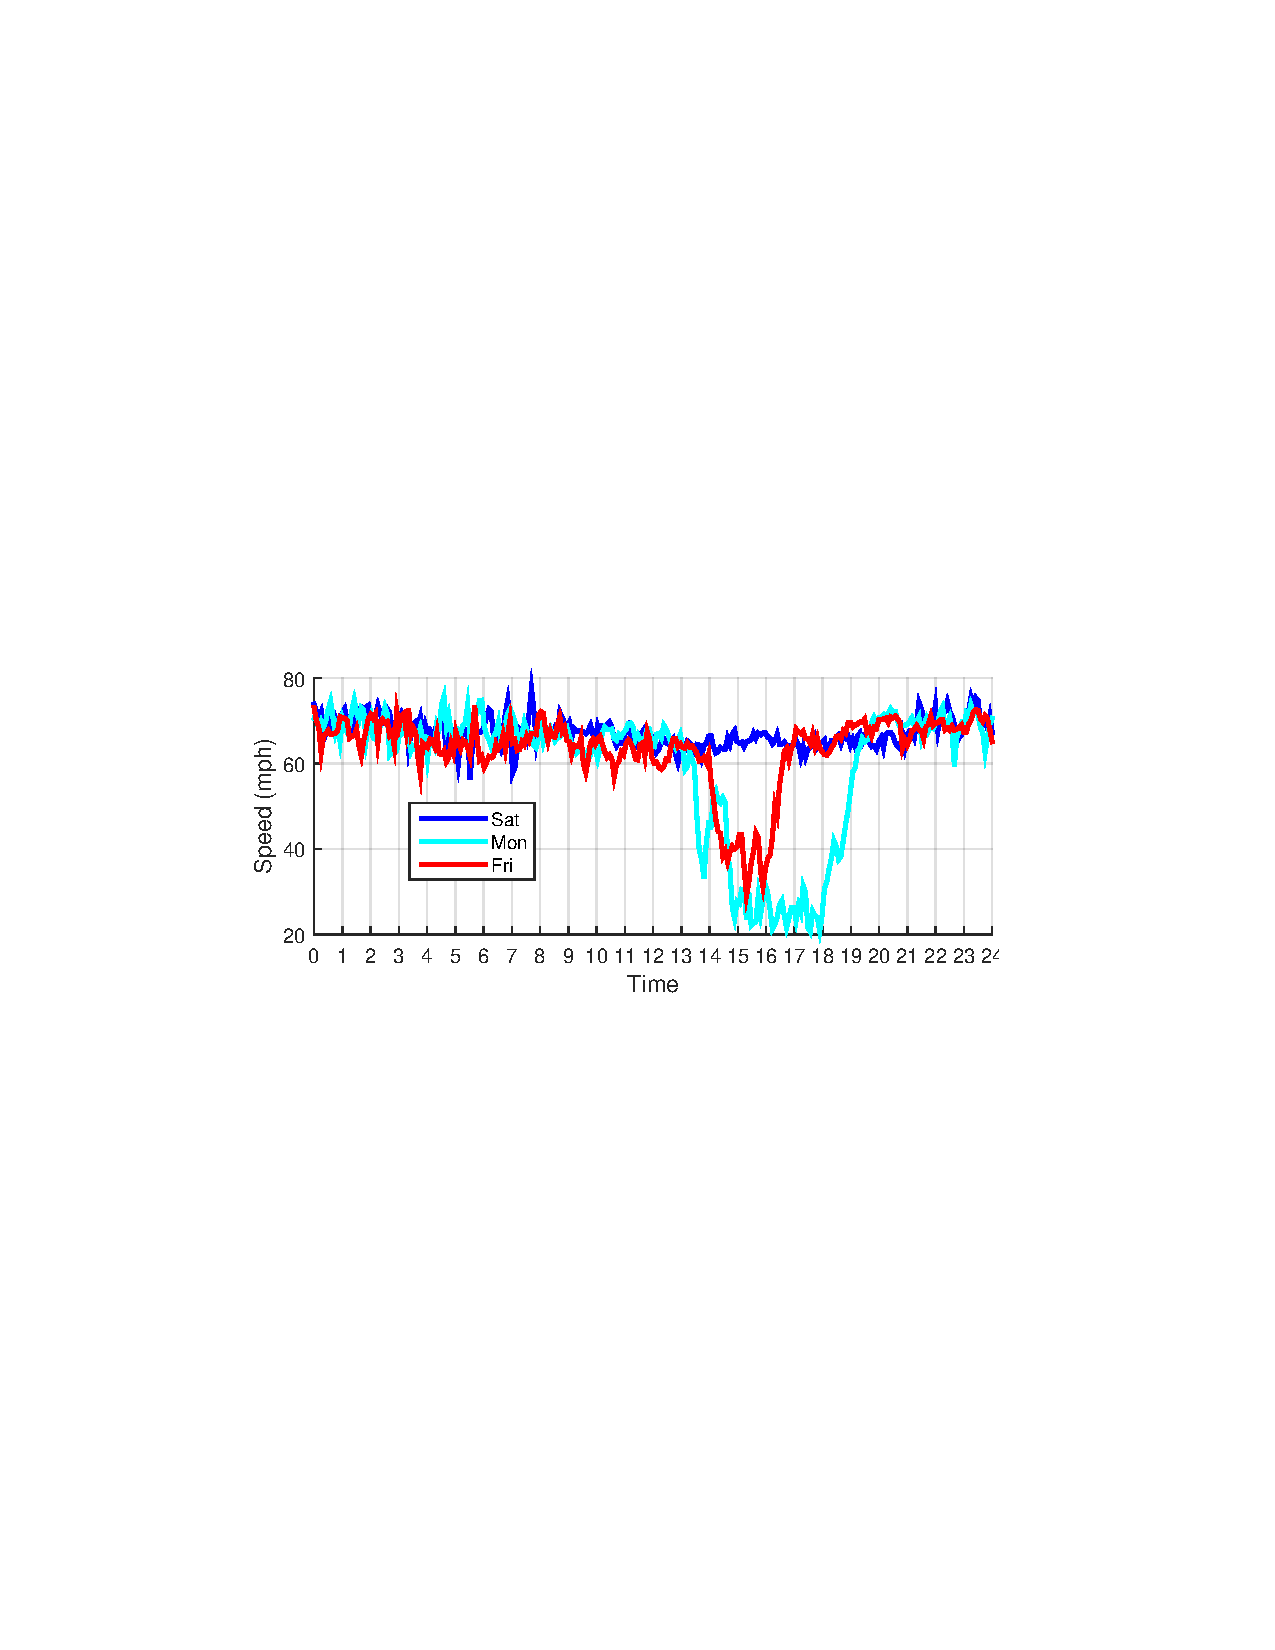
\includegraphics[width=0.7\linewidth]{./Figures/spd1}
	\caption{Average speed for three days.}
	\label{fig:spd1}
\end{figure} 

\begin{figure}[h]
	\centering
	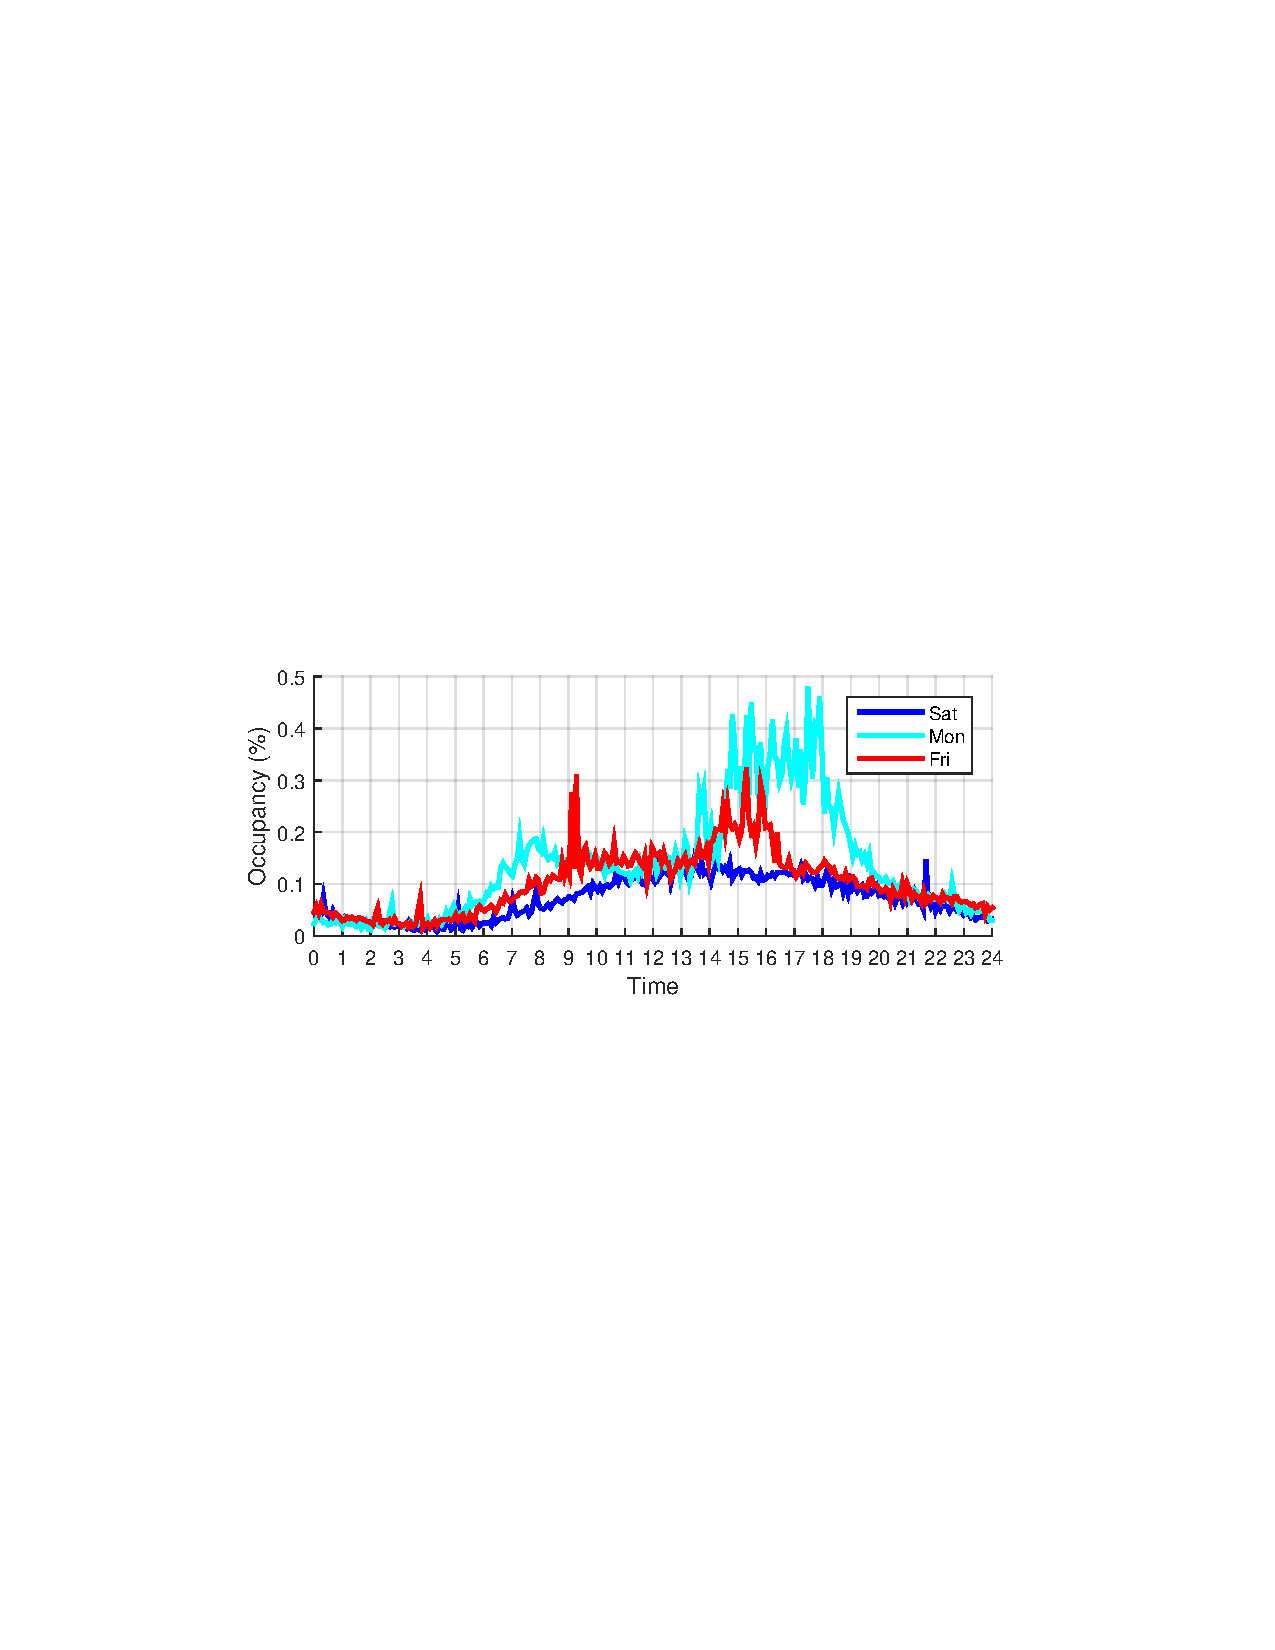
\includegraphics[width=0.7\linewidth]{./Figures/occ1}
	\caption{Average occupancy for three days.}
	\label{fig:occ1}
\end{figure} 

\begin{figure}[h]
	\centering
	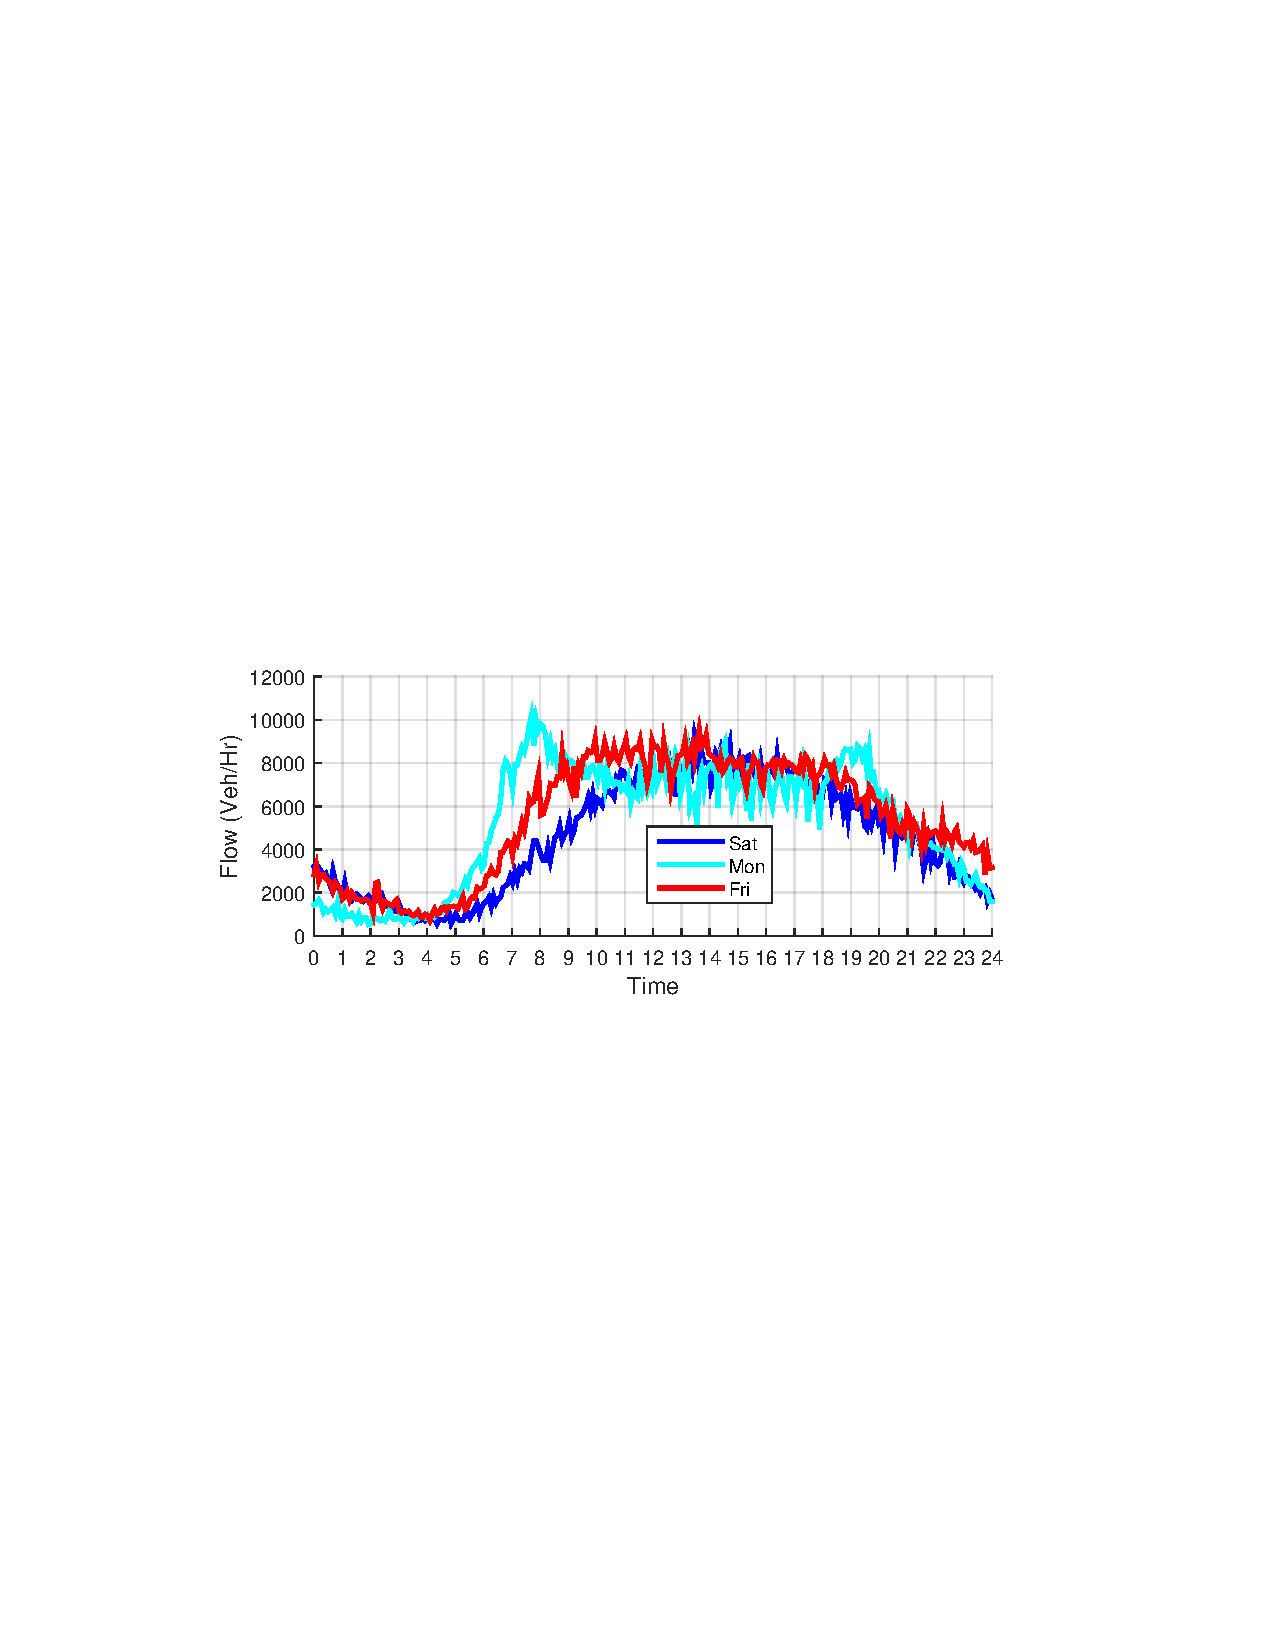
\includegraphics[width=0.7\linewidth]{./Figures/flw1}
	\caption{Average flow for three days.}
	\label{fig:flw1}
\end{figure} 
%\begin{figure}
%	\centering
%	\begin{subfigure}[b]{\linewidth}
%		\centering
%		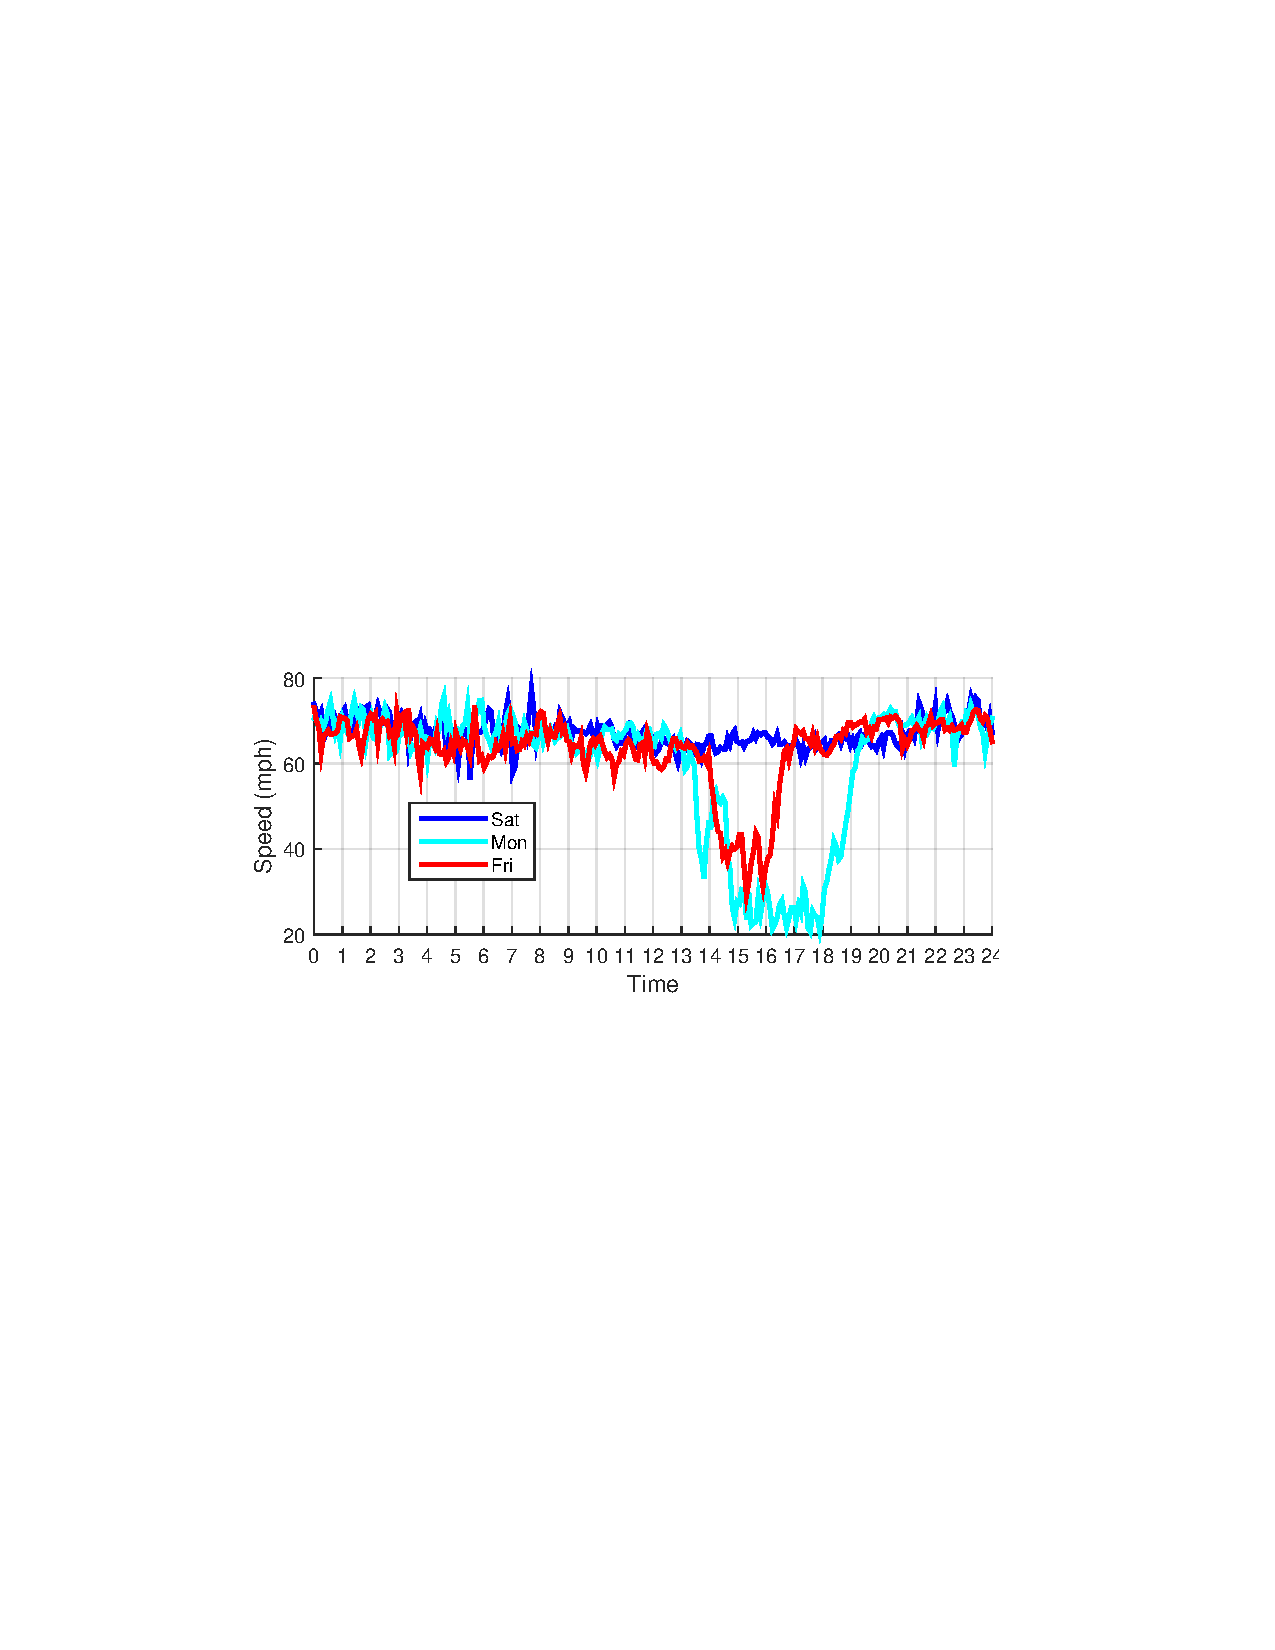
\includegraphics[width=0.69\linewidth]{./Figures/spd1}
%		%	\caption{Speed}
%		\label{fig:spd1}
%	\end{subfigure} 
%	\begin{subfigure}[b]{\linewidth}
%		\centering
%		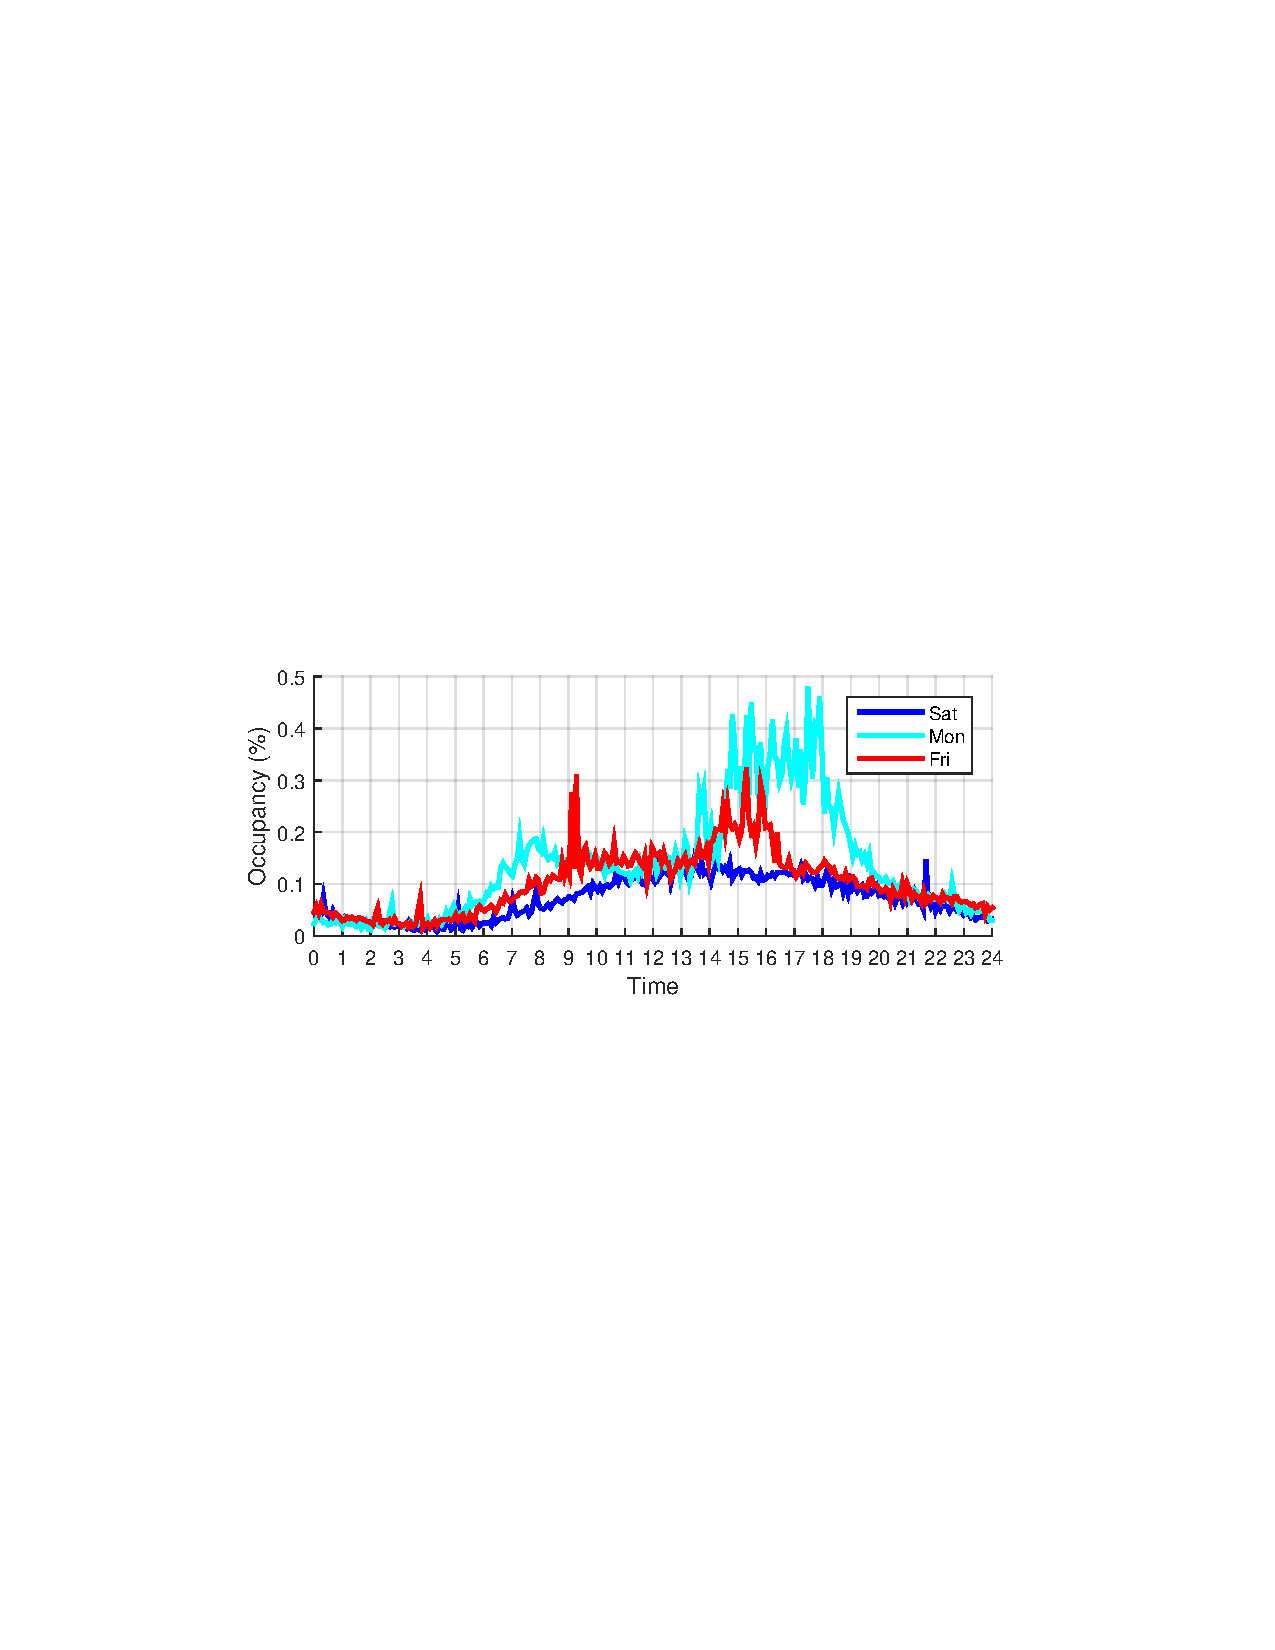
\includegraphics[width=0.69\linewidth]{./Figures/occ1}
%		%	\caption{Speed}
%		\label{fig:occ1}
%	\end{subfigure} 
%	\begin{subfigure}[b]{\linewidth}
%		\centering
%		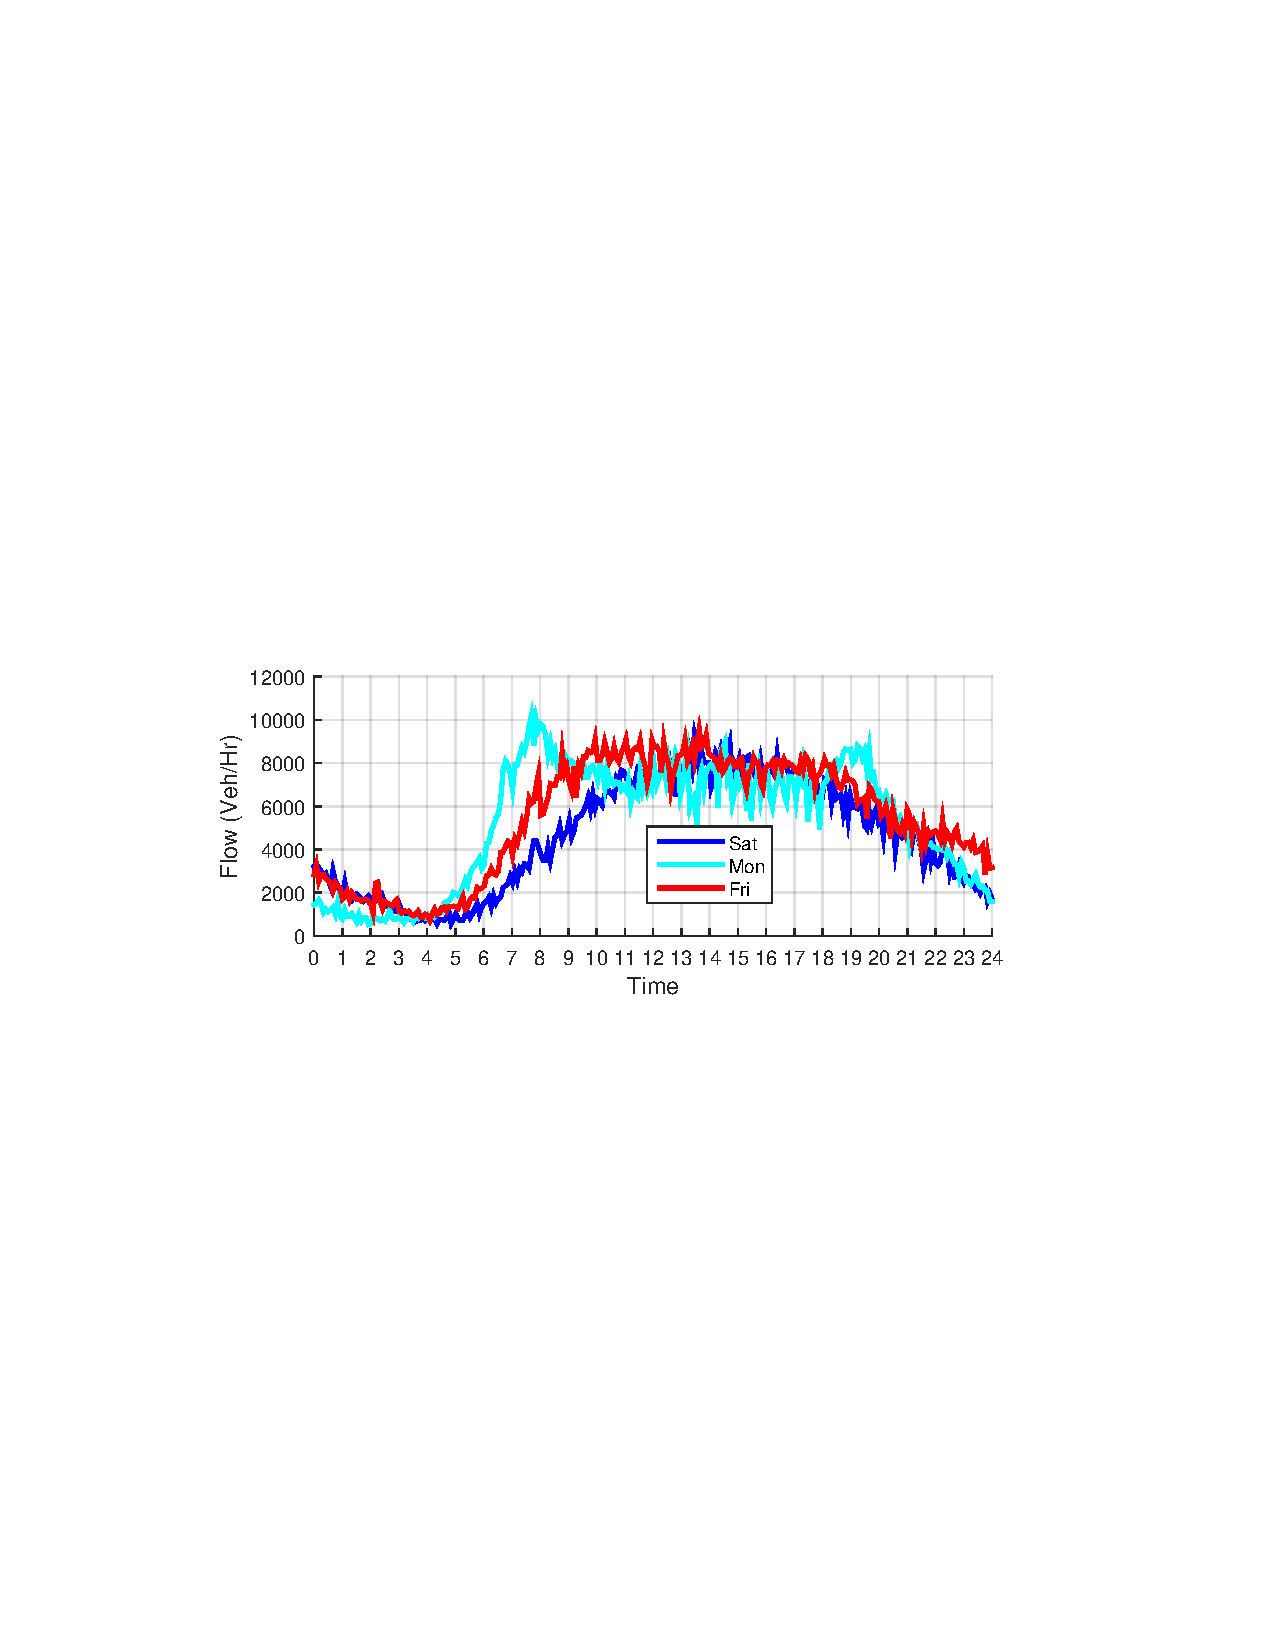
\includegraphics[width=0.7\linewidth]{./Figures/flw1}
%		\caption{Speed}
%		\label{fig:flw1}
%	\end{subfigure} 
%\end{figure}


Due to highly time-dependent nature of traffic, our training data for a single VDS (Vehicle Detection Station) in Freeway I-210 East is composed of the subsequent inputs:
\begin{itemize}
\item Flow
\item Occupancy
\item Speed
\item Date
\item Time of the day
\end{itemize}
 
\section{Training Method}
Our main focus of data training was obtaining one-step prediction of traffic behavior; in other words, giving the features of a particular time step of a specific day as the inputs, the outputs should be flow, speed and occupancy of the considered VDS in the next time step. In order to get such a prediction function, a multi-layer neural network was trained on the data, whose characteristics such as number of hidden nodes and number of hidden layers were obtained by cross-validation over a range of node numbers and number of layers.

\subsection{Neural Network Layout}

\begin{figure}[t]
	\centering
	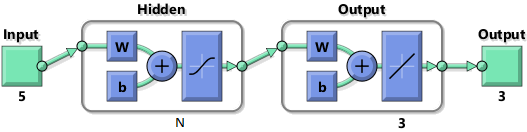
\includegraphics[width=1\linewidth]{./Figures/NN_1}
	\caption{Initial neural-network layout with one hidden and one output layer that have \emph{tanh} and \emph{linear} activation functions respectively. }
	\label{fig:nn1}
\end{figure} 


\begin{figure}[t]
	\centering
	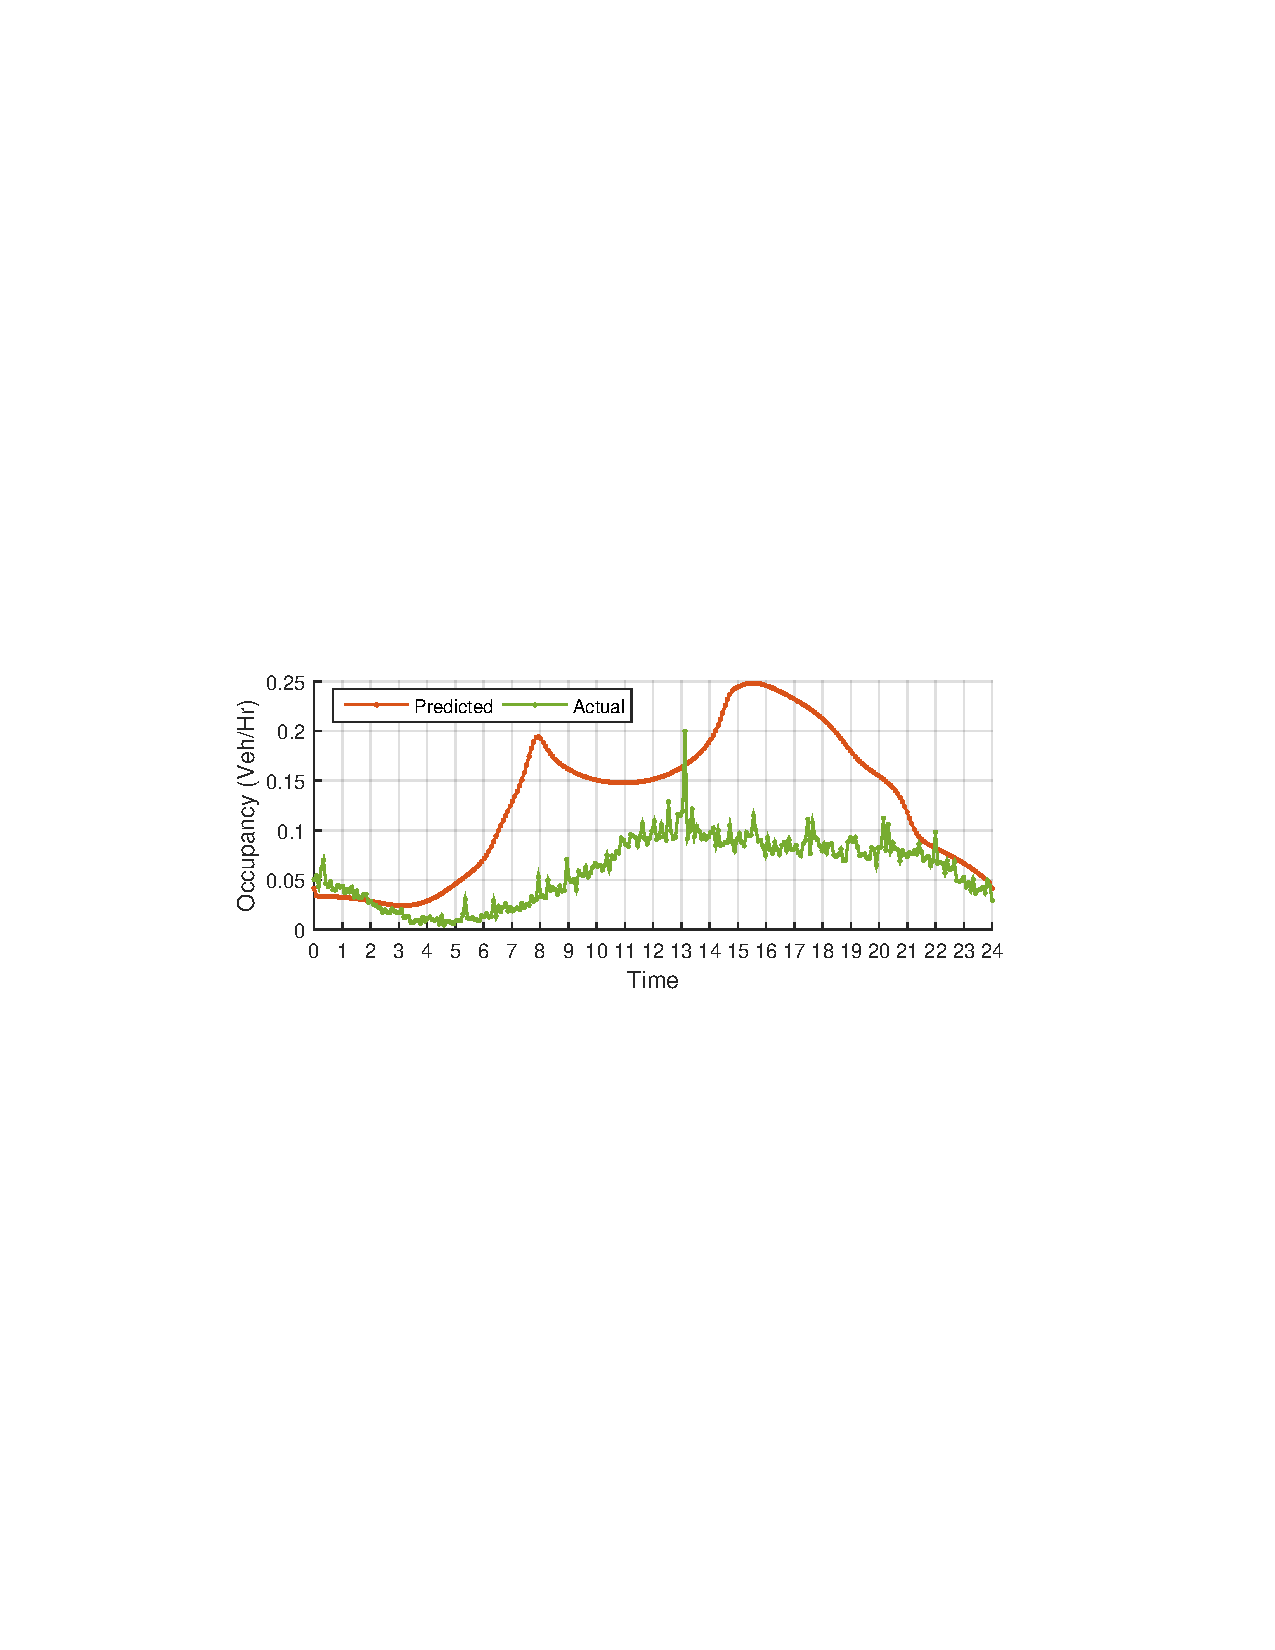
\includegraphics[width=0.7\linewidth]{./Figures/badPrediction}
	\caption{An example of ``bad'' prediction on a Wednesday: the predicted occupancy based on the initial states differs from the actual occupancy values reported by VDS during the day.}
	\label{fig:badPrediction}
\end{figure}


It is known by Universal Approximation Theorem  \cite{universality} that any continuous function on a bounded domain can be approximated by a two-layer neural network with a finite number of hidden nodes. Thereby, the very first step in implementing a NN (deep) learning algorithm is to start with a neural network that has one hidden layer and one output layer as is shown in Fig.~\ref{fig:nn1}. 

In such an architecture, there are three crucial design parameters, namely the number of nodes in the hidden layer, the activation functions for the nodes and the cost function that is desired to be minimized when the trained network is applied to test data. In our running example, the number of nodes in the output layer is 3 since the output vector contains the measurements of \emph{flow}, \emph{occupancy} and \emph{speed}. The input vector, here, contains the same signals with one step delay as well as the corresponding time and day number (i.e. a vector in $\mathbb{R}^5$). 

As mentioned above, a design parameter determining structure of the network is number of hidden nodes, denoted by $N$ in Fig.~\ref{fig:nn1}, that should be determined prior to the training process. In order to decide on the ``optimal'' number of hidden nodes, a range of values from $2$ to $80$ was chosen. We considered \emph{tanh} as the activation function for the neurons in the hidden layer, and a pure \emph{linear} function for the output layer nodes (c.f. Fig.~\ref{fig:nn1}). 

There are many different algorithms such as ``Levenberg-Marquardt'' and ``Scaled Conjugate Gradient'' that can be used for training neural networks. Choosing the right algorithm may be a tedious process since it depends on many factors, including the complexity of the problem, the number of data points in the training set, the number of weights and biases in the network, the error goal, and whether the network is being used for pattern recognition (discriminant analysis) or function approximation (regression). Here, we started off with Levenberg-Marquardt backpropagation \cite{hagan1994training} since it is often one of the fastest backpropagation algorithms for regression, and it is usually recommended as a first-choice supervised algorithm.
Like the quasi-Newton methods, the Levenberg-Marquardt algorithm was designed to approach second-order training speed without having to compute the Hessian matrix. 
We chose MSE (mean squared error) as the optimization cost function. Validation vectors are used to stop training early if the network performance on the validation vectors fails to improve or remains the same for ``max-fail'' epochs in a row. Test vectors are used as a further check that the network is generalizing well, but do not have any effect on training. In MATLAB, training stops when any of these conditions occurs:
\begin{enumerate}
\item The maximum number of epochs (repetitions) is reached.
\item The maximum amount of time is exceeded.
\item Performance is minimized to the goal.
\item The performance gradient falls below min-grad.
\item $\mu$ exceeds $\mu_{\max}$.
\item Validation performance has increased more than max-fail times since the last time it decreased (when using validation).
\end{enumerate}

\subsection{Initial Results:}\label{sec:initial}
We used MATLAB to train a neural network with the aforementioned parameters and architecture. Once our first predictor, say $M$, was trained, we applied it to the testing set as follows. The initial input to the neural network for a particular day, say $d$, and initial time, say $k_0$, was the state measurements -- flow ($f$), speed($s$), occupancy($o$), day number and time -- and the output was the prediction of flow, speed and occupancy in the next 5 minutes. 
\begin{align}
\begin{bmatrix}
\hat{f}(k_0+1)\\\hat{s}(k_0+1)\\\hat{o}(k_0+1)
\end{bmatrix} = M(f(k_0),s(k_0), o(k_0), k_0, d)
\end{align}
In the next step, we used these predicted values with corresponding time (previous time plus 5 minutes) and the same day number as the inputs for the next prediction
\begin{align}
\begin{bmatrix}
\hat{f}(k+1)\\\hat{s}(k+1)\\\hat{o}(k+1)
\end{bmatrix} = M(\hat{f}(k),\hat{s}(k), \hat{o}(k), k, d), \quad k_0<k\le k_0+H.
\end{align}
Here, $H$ is the maximum number of step that keeps time $k_0+H$ still in the same day $d$. By visualization of the prediction error we observed that the accuracy results for some days is very poor. We call these days ``unusual'' and expect that this irregularity is due to special circumstances such as very different weather conditions, road constructions or holidays. An example of this type of bad predictions is shown in Fig.~\ref{fig:badPrediction}.

\subsection{Classification of Days Using Unsupervised Learning:}
Being motivated by removing the ``unusual'' days (bad data) from the data set in an automatic manner, we propose categorizing the days into twofolds using an unsupervised clustering algorithm since there is no label available for usual and unusual days. We used K-means clustering with increasing value of $k$ (i.e. number of clusters) starting from $k=1$. Our strategy for finding the best number of clusters is that for each choose of $k$ we define the ``usual'' days as the instances that form the most crowded cluster, and label the other instances as ''unusual" days. It is clear that if $k$ is very large, the total distance will be very small but the number of useful data points labeled as ''usual" days will be also decreased. Therefore, we should look for the smallest value of $k$ that does not create a small cluster of useful data set. Therefore, we define the best value of $k$ as the smallest positive integer that decreases the total distance of data points that decreases the total distance by a factor of $c$ and at the same time labels at least $b\%$ of data points as the ``usual" days. After a few manual iterations, we chose $c=1.1$ and $b=90$. Using these two values, all days were either classified to two clusters (good and bad data), or one cluster -- all data was useful for that particular weekday, e.g. Mondays. In a preprocessing stage we normalized the flow, speed and occupancy data to have zero mean and unit variance and then stuck them together to create one single vector in $\mathbb{R}^{864}$ ($288$ samples for each of these three signals). An example of clustering results is shown in Fig.~\ref{fig:clustering} where the data of occupancy of all Wednesdays is categorized into usual and unusual days.

\begin{figure}[t]
	\centering
	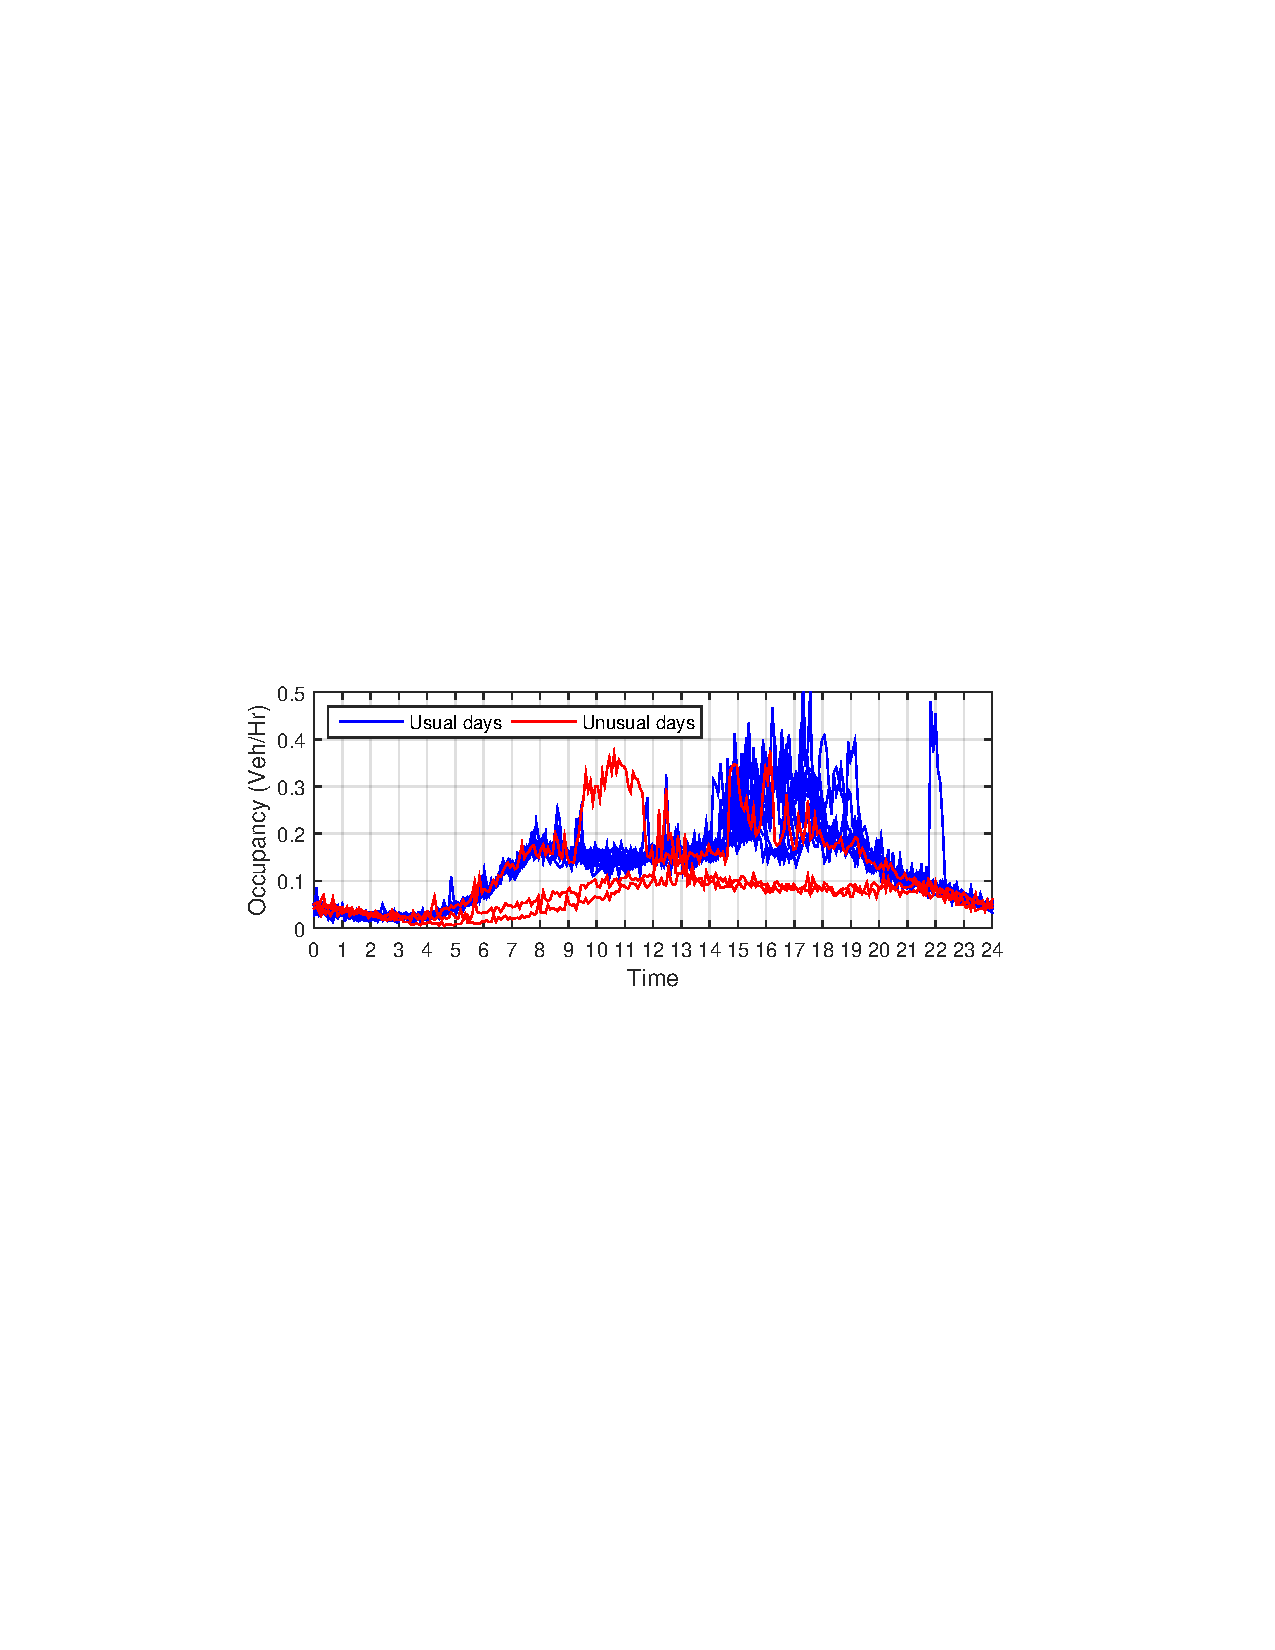
\includegraphics[width=0.8\linewidth]{./Figures/clustering}
	\caption{An unsupervised clustering example for separating data of Wednesdays to ``usual'' and ``unusual'' days using K-Means.}
	\label{fig:clustering}
\end{figure}

\subsection{Final Results}
Training on data of usual days for a the same number of neurons as section \ref{sec:initial} is performed with different random initializations to avoid being trapped in local minima and the performance of trained network is shown in Fig~\ref{fig:perf1}. This figure indicates that the best performance is achieved by approximately $50$ nodes in the hidden layer when the activation function is \textit{tanh}. Larger number of nodes  in this particular case results in a smaller training error, but at the same time causes over-fitting. The number of network parameters being learned by this network is 453 $\left([5+1]\times50+[50+1]\times 3\right)$.
\begin{figure}[t]
	\centering
	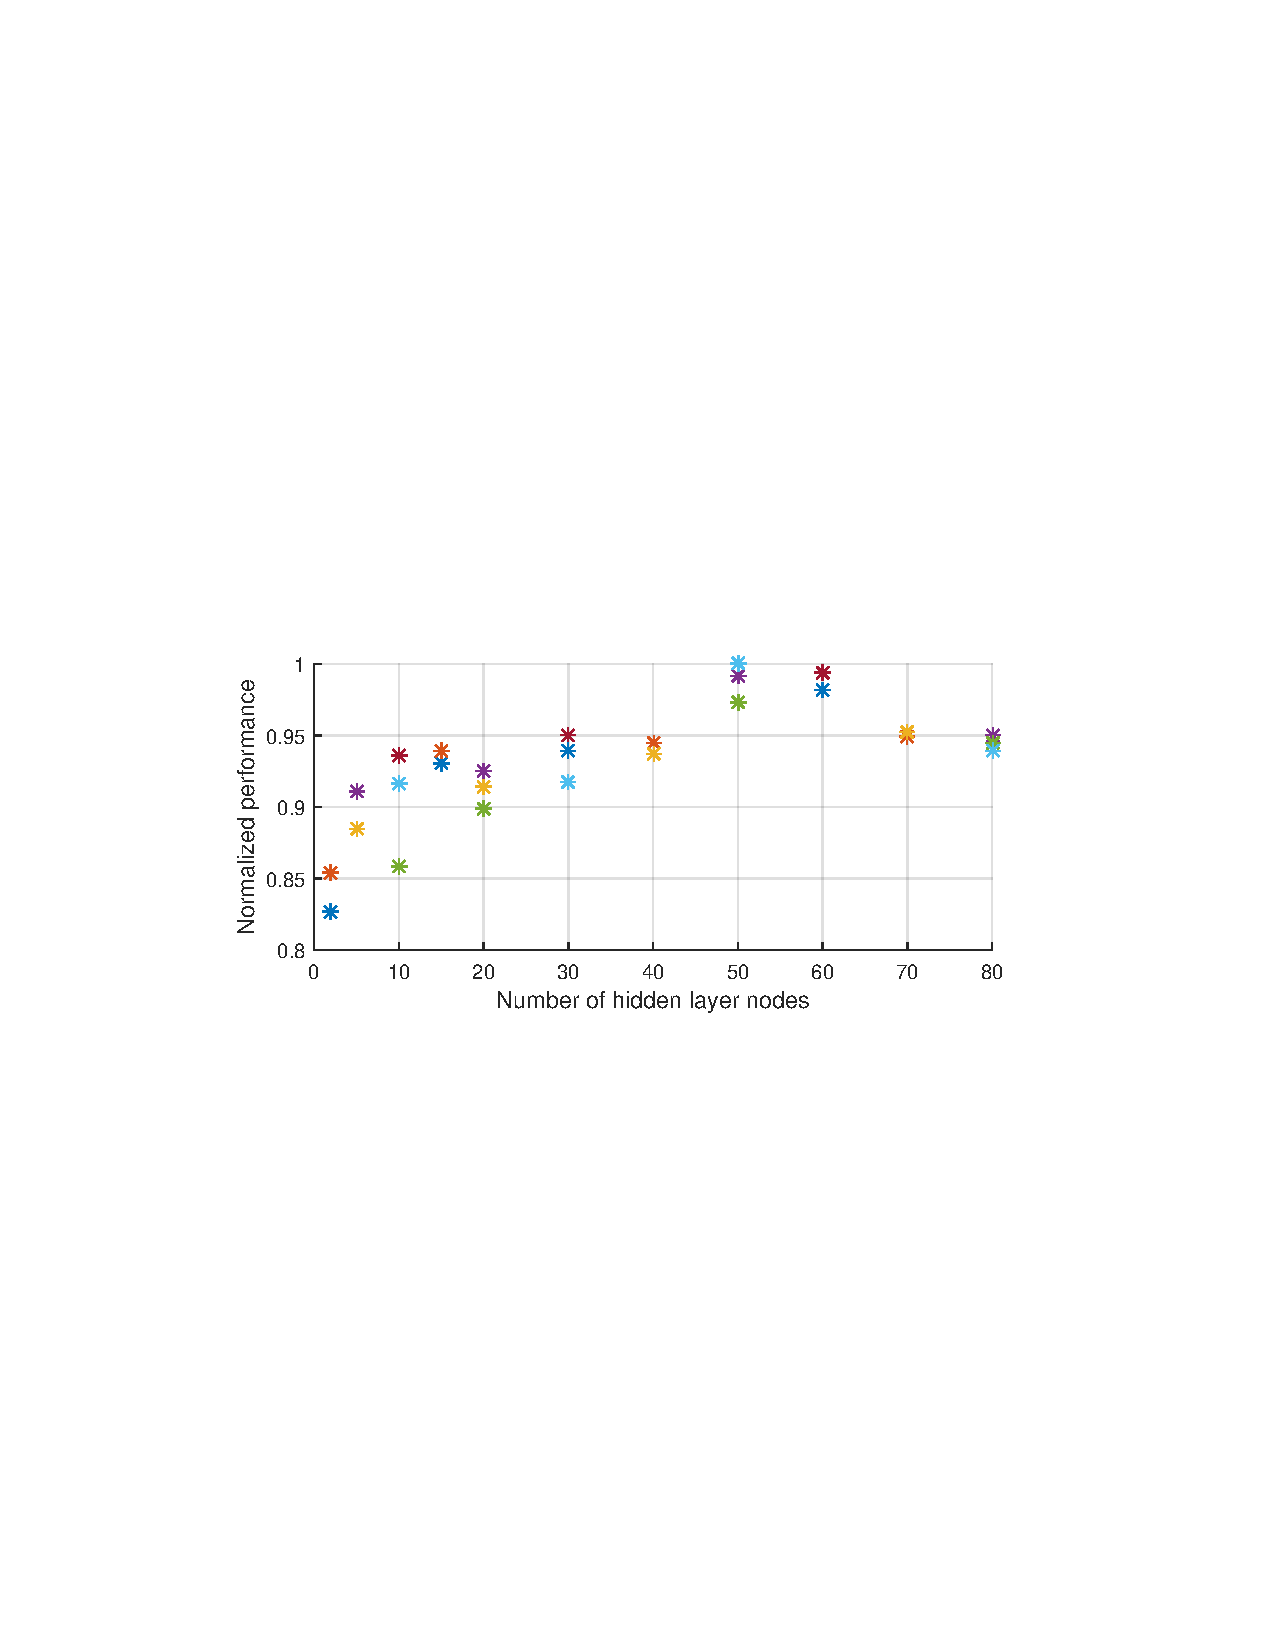
\includegraphics[width=1\linewidth]{./Figures/perf1}
	\caption{ The performance of trained neural network being normalized by the maximum achieved performance versus the number of nodes in the hidden layer when \emph{tanh} and \emph{linear} activation functions are used. }
	\label{fig:perf1}
\end{figure} 
We also considered other activation functions including radial basis and sigmoid and repeated the process with the same design parameters (i.e. architecture and algorithm) and it was realized that among all \textit{tanh} performed better. Moreover, ``Scaled Conjugate Gradient'' (conjugate gradient backpropagation with Polak-Ribiére updates) \cite{moller1993scaled} and ``Variable Learning Rate Backpropagation'' (gradient descent with momentum and adaptive learning rate backpropagation) were considered as alternative algorithms. Among these three algorithms, Levenberg-Marquardt had the fastest convergence rate and smallest mean squared error. The set of all designing parameters used in the ``best'' achieved training are listed in Table~\ref{tab:param}. The code was being run in MATLAB on a machine with Windows Server 2012, Intel(R) Core(TM) i7-3770 CPU and 12.0 GB of RAM. Parallel computing toolbox of MATLAB was used to utilize 4 workers in a parallel pool for the training process. The total training time in this environment for the best case was 88 seconds. The mean squared error evolution during the training for train, validation and test set is shown in Fig.~\ref{fig:trainingPerf}.

\begin{table}[t]
	\centering

	\caption{Final parameters used for neural network training}
\begin{tabular}{c|c}	
	\hline
	\hline Algorithm & Levenberg-Marquardt \\ 
	\hline Number of layers / parameters & 2 / 453 \\ 
	\hline MSE (normalized input/output ) & 0.051 \\ 
	\hline Number of epochs (time) & 117 (88 seconds) \\ 
	\hline  	 
\end{tabular} \label{tab:param}
\end{table}

\begin{figure}[t]
	\centering
	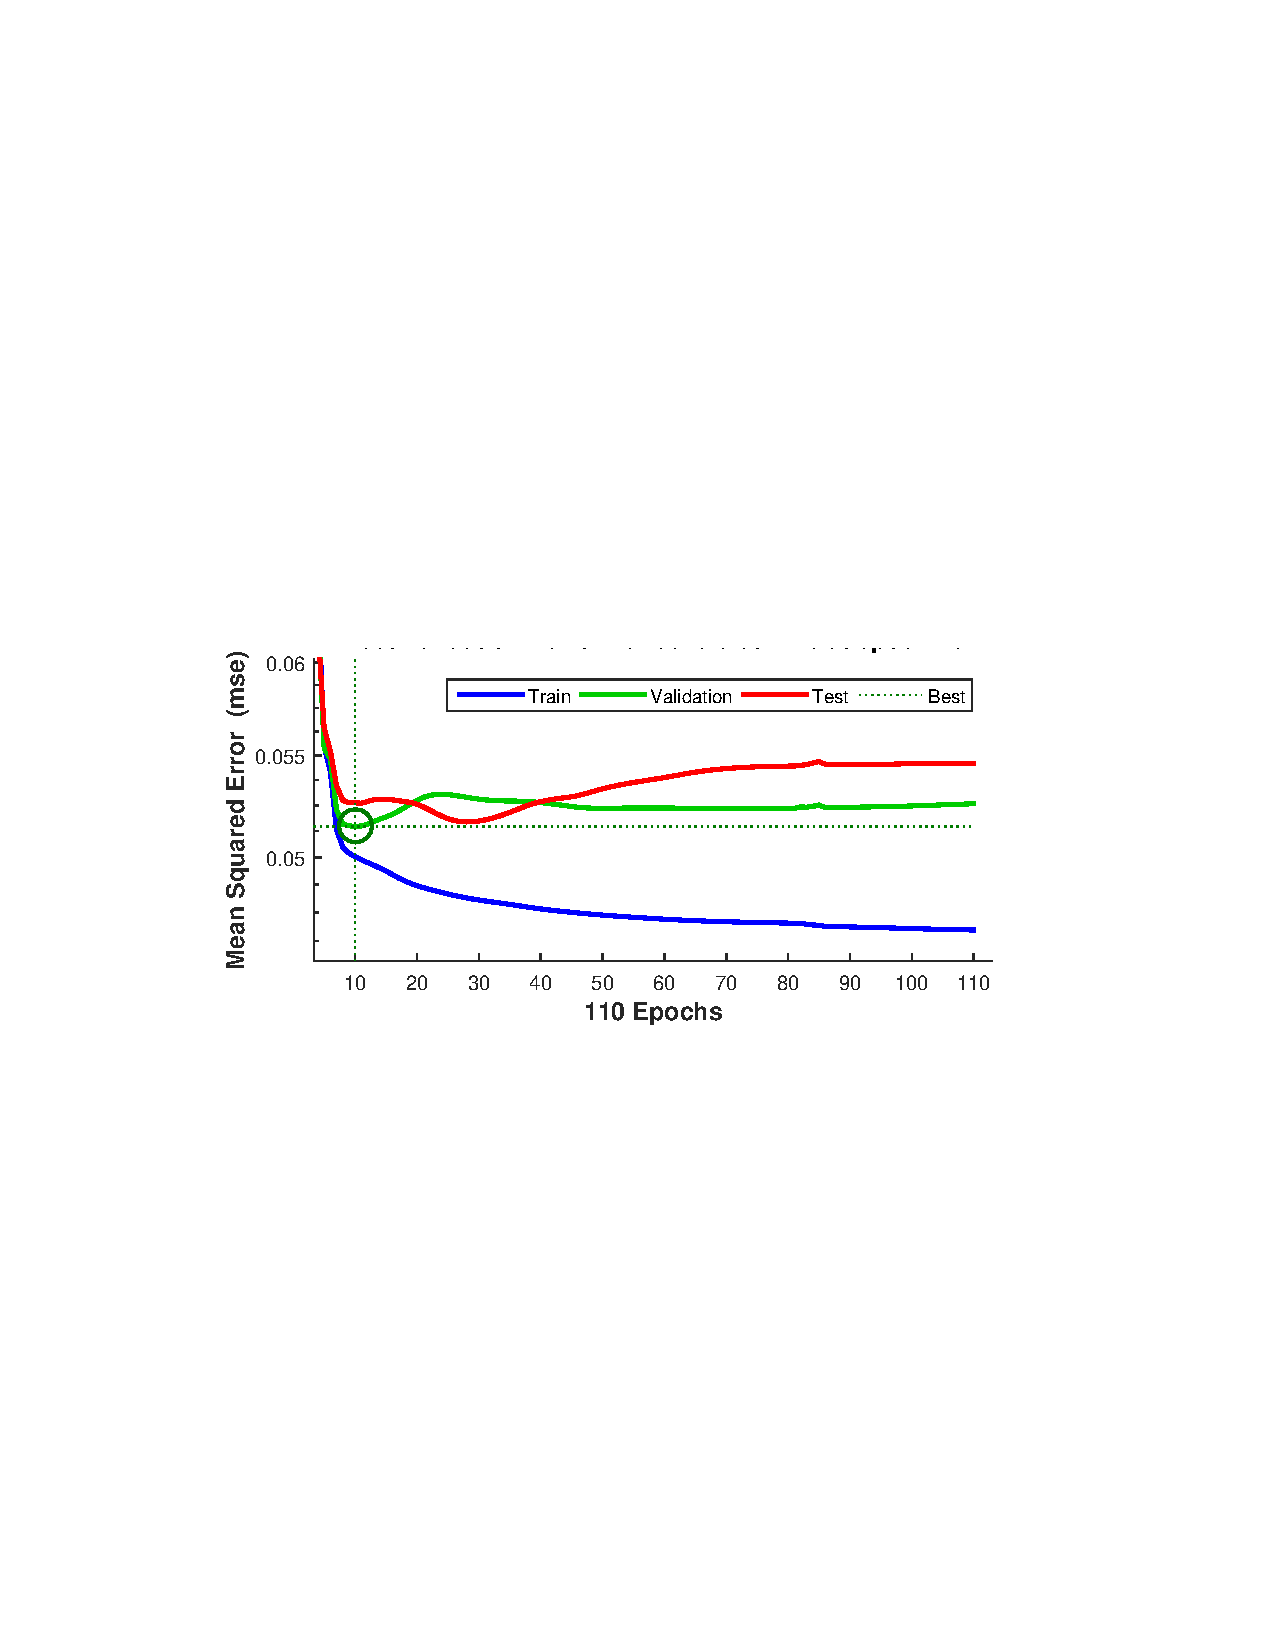
\includegraphics[width=1\linewidth]{./Figures/trainingPerf}
	\caption{ Training, validation and test performance. }
	\label{fig:trainingPerf}
\end{figure}

The trained neural network is used for short-time traffic prediction which is in fact our ultimate objective in this paper. As mentioned multiple times throughout the paper, the actual traffic states are sampled every 5 minutes by PeMS. Here, we are interested to know how our trained neural network is able to predict data when this fine resolution is not available. This is being tested by injecting the actual state to the model and then predicting the next 12 steps (60 minutes) without having access to the actual data till it will receive the next sample. Figure~\ref{fig:final1} depicts the actual and predicted data for Sat, Oct-04-2014 and Mon, Oct-06-2014. As can be seen in the figure, each predicted plot contains 24 small jumps that correspond to the moments the actual data is fed back to the predictor. As can be seen from the figure, the predicted data between these samples matches the real values very well.
\begin{figure}[t]
	\centering
	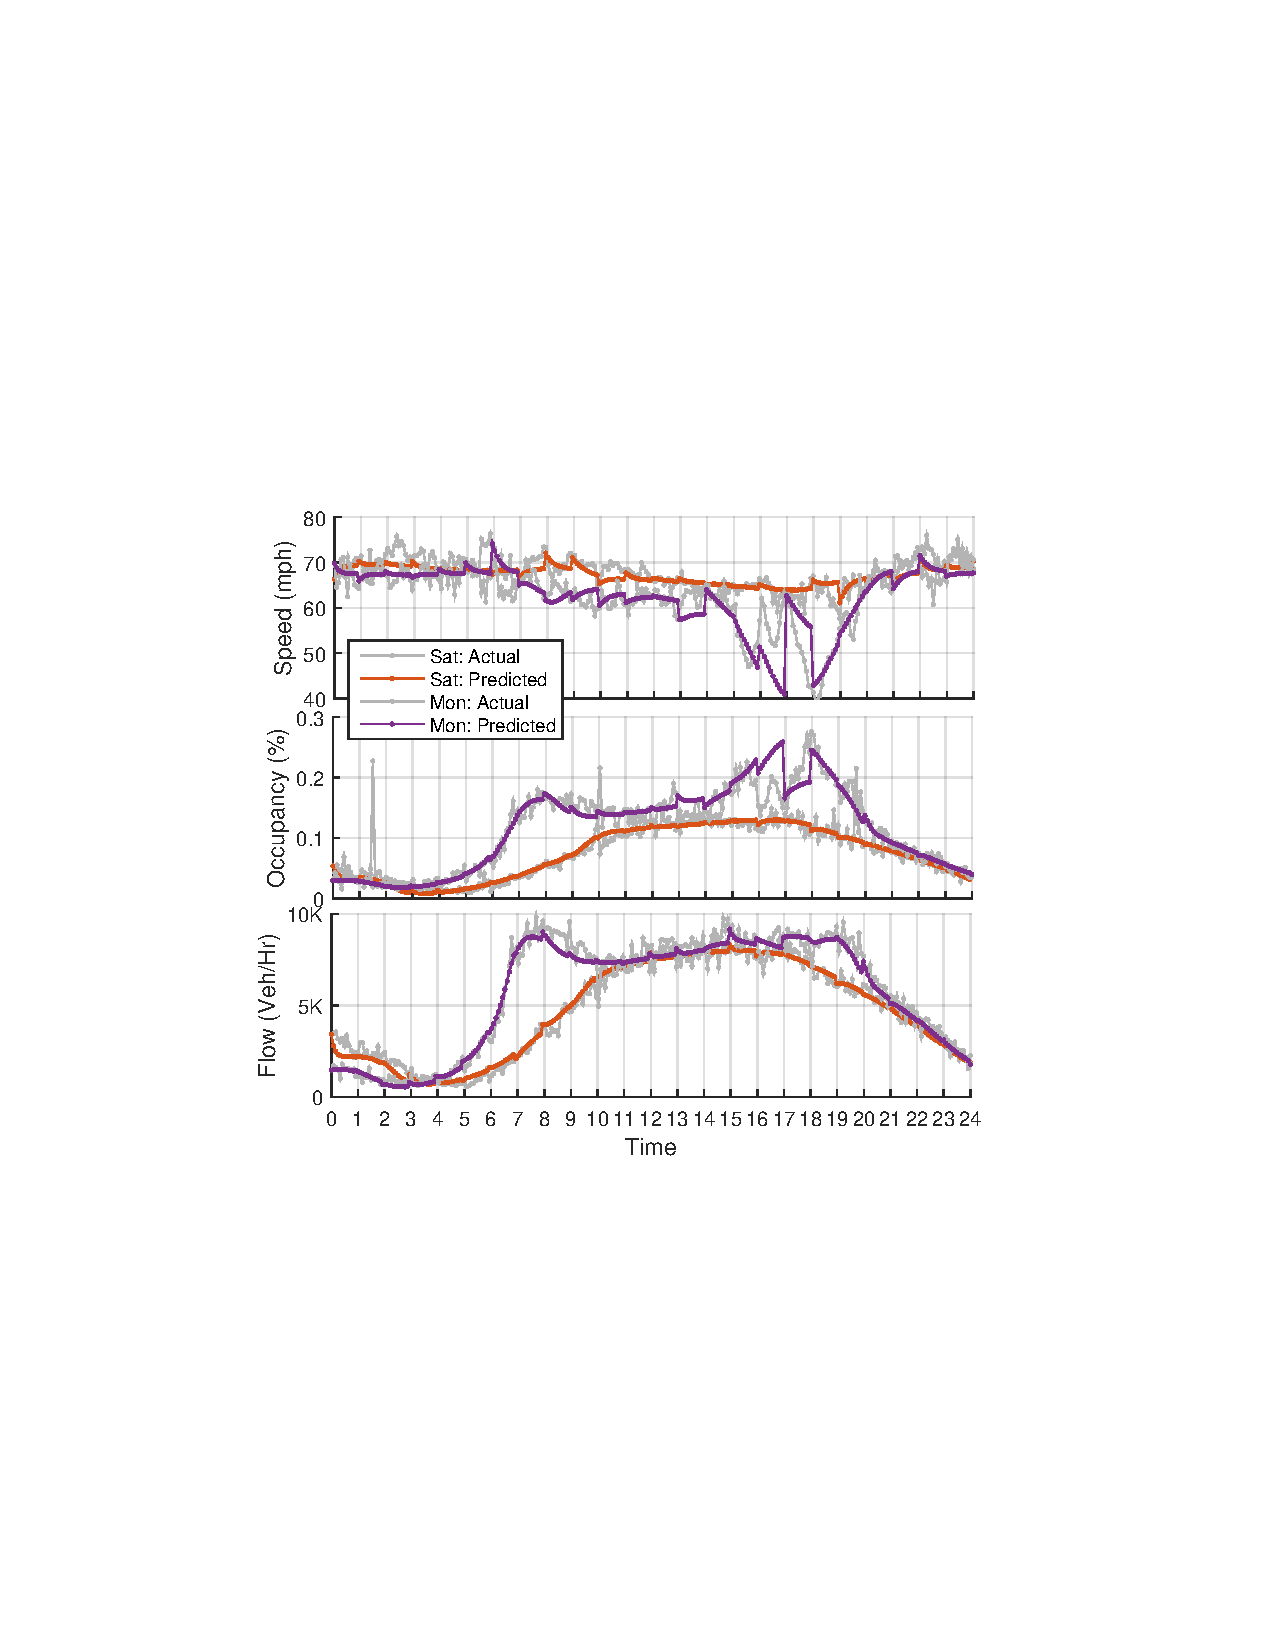
\includegraphics[width=1\linewidth]{./Figures/final1}
	\caption{Actual and predicted traffic data on Sat, Oct-04-2014 and Mon, Oct-06-2014. Predictor has received actual data every 1 hour (jumps on the plot) and predicted traffic states every 5 minutes till the next sampling arrives.}
	\label{fig:final1}
\end{figure}

The next step is determination of number of layers in the desired network. The question of what is the best of way of configuring a particular number of nodes (in this case $50$) should be addressed. Evidently, best in the optimal sense is obtained by optimizing over the whole set of possible configurations of the network which is practically impossible; hence, performance of several configurations of the network with $50$ nodes is compared (figure \ref{}) where the best performance is obtained by $x$ number of layers where first layer has $x$ number of nodes...

 
\section{Conclusion and Future Work}
A fully automated scheme for predicting freeway traffic data by deploying neural networks was proposed. 
Our scheme had two main steps, namely detecting ``unusual" measurements and removing them in a preprocessing stage, and training a two layer neural network based on the real traffic data provided by PeMS.
Since usual and unusual days, by our definition, are not labeled we used an unsupervised classification algorithm with a self adjusting number of clusters to separate ``unusual" days from ``usual" days. A comprehensive study on  different possibilities for the architecture of neural network and training algorithm was performed. However, we did not present a deep learner by utilizing multilayer neural networks. Hence, this can be considered in a future work. Another interesting aspect of this problem that can be investigated is predicting traffic data in what we called ``unusual" days.

\bibliographystyle{plain}
\bibliography{references}

%%%%%%%%%%%%%%%%%%%%%%%%%%%%%%%%%%%%%%%%%%%%%%%%%%%%%%%%%%%%%%%%%%%%%%
%\appendix       %%% starting appendix
%\section*{Appendix A: Head of First Appendix}
%Avoid Appendices if possible.
\




\end{document}
